% THIS IS AN EXAMPLE DOCUMENT FOR VLDB 2012
% based on ACM SIGPROC-SP.TEX VERSION 2.7
% Modified by  Gerald Weber <gerald@cs.auckland.ac.nz>
% Removed the requirement to include *bbl file in here. (AhmetSacan, Sep2012)
% Fixed the equation on page 3 to prevent line overflow. (AhmetSacan, Sep2012)

\documentclass{vldb}
\usepackage{graphicx}
\usepackage{balance}  % for  \balance command ON LAST PAGE  (only there!)


\begin{document}

% ****************** TITLE ****************************************

\title{Deep Convolutional Neural Network for Spatial Temporal Human Action Recognition}

% possible, but not really needed or used for PVLDB:
%\subtitle{[Extended Abstract]
%\titlenote{A full version of this paper is available as\textit{Author's Guide to Preparing ACM SIG Proceedings Using \LaTeX$2_\epsilon$\ and BibTeX} at \texttt{www.acm.org/eaddress.htm}}}

% ****************** AUTHORS **************************************

% You need the command \numberofauthors to handle the 'placement
% and alignment' of the authors beneath the title.
%
% For aesthetic reasons, we recommend 'three authors at a time'
% i.e. three 'name/affiliation blocks' be placed beneath the title.
%
% NOTE: You are NOT restricted in how many 'rows' of
% "name/affiliations" may appear. We just ask that you restrict
% the number of 'columns' to three.
%
% Because of the available 'opening page real-estate'
% we ask you to refrain from putting more than six authors
% (two rows with three columns) beneath the article title.
% More than six makes the first-page appear very cluttered indeed.
%
% Use the \alignauthor commands to handle the names
% and affiliations for an 'aesthetic maximum' of six authors.
% Add names, affiliations, addresses for
% the seventh etc. author(s) as the argument for the
% \additionalauthors command.
% These 'additional authors' will be output/set for you
% without further effort on your part as the last section in
% the body of your article BEFORE References or any Appendices.

\numberofauthors{1} %  in this sample file, there are a *total*
% of EIGHT authors. SIX appear on the 'first-page' (for formatting
% reasons) and the remaining two appear in the \additionalauthors section.

\author{
% You can go ahead and credit any number of authors here,
% e.g. one 'row of three' or two rows (consisting of one row of three
% and a second row of one, two or three).
%
% The command \alignauthor (no curly braces needed) should
% precede each author name, affiliation/snail-mail address and
% e-mail address. Additionally, tag each line of
% affiliation/address with \affaddr, and tag the
% e-mail address with \email.
%
% 1st. author
\alignauthor
Sami Arja\titlenote{~Indicate first author.}\\
       \affaddr{Western Sydney University}\\
       \affaddr{School of Computing, Engineering and Mathematics}\\
       \email{18040571@westernsydney.edu.au}\\
       \email{Advisor: Professor Gu Fang \titlenote{Indicate principle supervisor.}}
% 2nd. author
\alignauthor
Dr. Gu Fang
       \affaddr{Western Sydney University}\\
       \affaddr{School of Computing, Engineering and Mathematics}\\
       \email{G.fang@westernsydney.edu.au}
}

% There's nothing stopping you putting the seventh, eighth, etc.
% author on the opening page (as the 'third row') but we ask,
% for aesthetic re
\date{30 July 1999}
% Just remember to make sure that the TOTAL number of authors
% is the number that will appear on the first page PLUS the
% number that will appear in the \additionalauthors section.


\maketitle

\begin{abstract}

Deep Learning is a very important task in human action recognition (HAR), as it has solved very complicated applications due to the rise of high quality software and hardware configurations with increasing in accuracy over time. Nevertheless, HAR has been one of the challenging tasks in computer vision due to the complexity of video data and the scarcity and lack of labelling and annotations. In this paper, we proposed two neural networks for action detection based on a sequence of frames in videos. These networks are conjoined deep learning models that are able to identify and localize actions based on their 3D convolution characteristics which are used to regress and classify an action of interest in videos. The robustness of the proposed architectures is compared amongst benchmark results. We employed these models to the challenging fine-grained KTH datasets and exhibited substantial improvements over the state of the art results with an accuracy as high as 92.23\%.

\end{abstract}

\section{Introduction}
Teaching robots to recognise human actions in videos is the primary research problem in computer vision. It can be implemented at different levels of abstraction. In the field of activity recognition, the focus is on identifying the individual characteristics of a particular action, to be used as a biometric cue. The main hierarchy is adopted by Moeslund \textit{et al.} \cite{moeslund2006survey}, where they divided actions to 4 main categories such as gesture, action and interaction and group activity. Gestures are the atomic movements that are less complex and take less time to perform. Actions, on the other hand, comprise a number of succeeding gestures and give an interpretation of the movement that is being performed. For example, "hand waving" is a gesture, whereas "walking" is an action. "jumping obstacles" is classified as an action, because it contains starting, jumping and running actions. Interactions are the types of activity performed in the existing of another object or human in the scene, for example, human riding a bicycle. Finally, group activity is performed by numbers of people and object, for example, people are walking in the shopping centre, this type of action takes a long time to perform and they are generally more complex.
 Different taxonomies have been proposed, Karpathy \textit{et al.} \cite{karpathy2014large} explore different frame-level method over time. Ng \textit{et al.} \cite{yue2015beyond} use recurrent neural network (RNN) alongside Convolutional neural network (CNN). Since these proposed methods relies only on frame based CNN features, the temporal information is not considered. Simonyan \textit{et al.} \cite{simonyan2014two} propose the two stream of CNN for HAR, which has a CNN that takes images as input and use optical flow in a separate network. Therefore, Wang \textit{et al.} \cite{wang2016actionness} extend on that and introduced an enhanced version of the dense trajectory (IDT) which is currently one of the handcrafted states of the art feature. The IDT descriptor as it has been claimed shows a good example of how the temporal signals can be handled in a different way than the spatial features. However, their approach is limited to computational power and the size of the dataset where the performance reduce if the dataset is unmanageably big, and even though they achieved great results, but these two factors still limit their possibility. Although, these methods take temporal feature as a separate stream shows promising performance for HAR application, however, they do not employ an end to end network and require two different computation stream. Ji \textit{et al.} \cite{ji20133d} propose a 3 dimensional CNN architecture a logical solution to this problem, that map the human action in videos based on their head tracking and body movement. Hou \textit{et al.} \cite{hou2017tube} introduced Tube CNN (T-CNN) for HAR that is capable of recognising and localising different actions based on their 3D convolutional characteristics, refer to Figure ~\ref{fig:T-CNN} for visualization. Tran \textit{et al.} \cite{tran2015learning} proposed 3D CNN for massive scale data, and shows that 3D layers outperform 2D CNN. Comparing these methods with each other, the 3D CNN approach \cite{ji20133d} is more closely linked to our proposed model. The segmented video volumes are used as inputs for the 3D CNN to classify actions. In contrast, our method takes the only frame where action exists and exclude all empty redundant frame to reduce complexity and unnecessary data.
\begin{figure*}
\centering
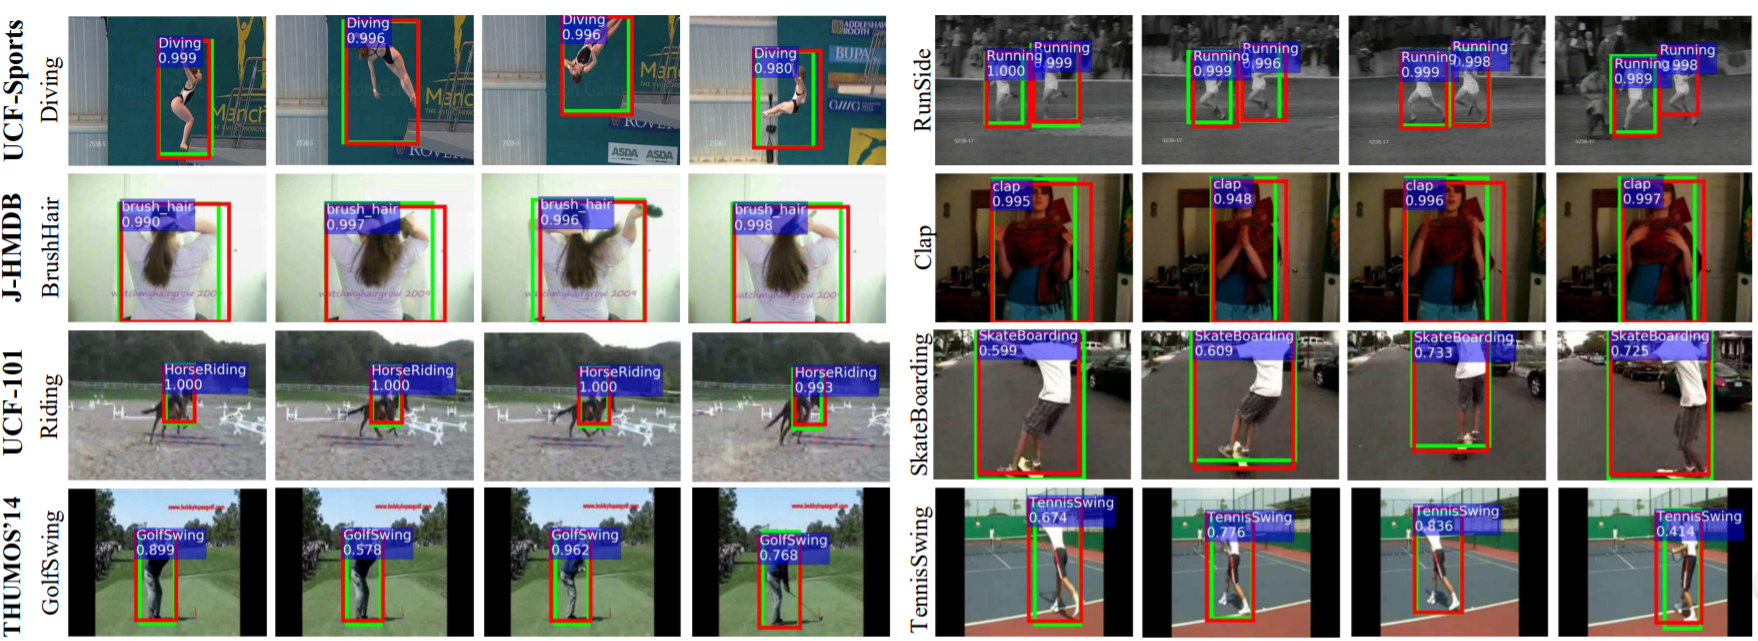
\includegraphics[width=2\columnwidth]{photo/trajectory1.PNG}
\caption{Action detection results from T-CNN on UCF sports, JHMDB, UCF-101 and THUMOS'14. The bounding box indicate the ground truth and the corresponding frames \cite{hou2017tube}}
\label{fig:T-CNN}
\end{figure*}


 Developing a fast and robust algorithm which can mimic this human identification capability can unlock great potentials. Some of its applications compromises in vigilance systems that involves man-machine interaction\cite{aggarwal2011human} \cite{kraiss2006advanced} , surveillance system \cite{roshtkhari2013human}, health-care \cite{chaaraoui2014evolutionary} and Video indexing and retrieval \cite{ramezani2016review}. In Human-Robot Interaction is applied where the efficiency of the robots/machines reach a high level of interaction in a cooperative practice. In Surveillance system, HAR is used in smart video monitoring systems that strives to automatically track the person and understand the performed activity, which helps in creating an automatic alert for direct reporting to the authority [5]
. In Healthcare, HAR is recently being used to understand patient activities and behaviours without using invasive and non-invasive sensors. Such an application has the potential to offer an objective, insightful service in clinical professionals. In Video indexing and retrieval HAR will aid in classifying videos based on their context rather than its features.

The aim of our research project is to build a system that can automatically assign semantic labels and descriptions to any input dataset, whether a video or static images where the human appear. Our proposed methods are designed in a view to narrow the gap between the low-level description and the given high-level representation. In this field, recognising human activity from a sequence of the video is a very important task, because the information about the people and the scene can be ultimately utilised to understand the action being executed.



\section{Materials and Methods}
We presented a study of action recognition accuracy for several forms of spatio-temporal network for video analysis. We used the dataset acquainted by Shnuld \textit{et al}.\cite{laptev2004recognizing}, and we used their results as benchmarks, as they are large enough to enable training of deep models. We developed a convolutional network model and we experimented its performance with regularization. In the end, we built a heterogeneous network consists of convolutional network with a Long short term memory (LSTM). 

\subsection{KTH Dataset}
KTH dataset is introduced by \cite{laptev2004recognizing}. This dataset is comprised of 6 types of human actions (refer to Figure \ref{fig:KTHdataset} for visualization). Actions being recorded are: Walking, Running, Jogging, Jumping, Hand waving and Hand clapping. There are 25 people involved in every action. There are 4 distinct scenarios for every action. Scenarios are outdoors, outdoors with scale variation, outdoors with different clothes and indoors. All recorded videos are taken over a consistent setting, their spatial resolutions are down-sampled to 120x160. A motionless camera is used to record the video sequences with 25 frames per second (fps) rate and has an average length of four seconds each. The AVI video file format is used to stored all videos sequences. There is a total of 599 videos for a combination of 25 subjects, 6 actions and 4 scenarios. KTH dataset offers major challenges, like illumination fluctuations, different people, obscurations, low resolution, scale variations, mixed scenarios, cloth variations, inter and intra action speed shifts.\\
\newline
\begin{figure}
\centering
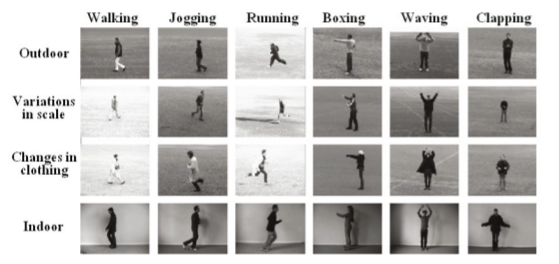
\includegraphics[width=0.95\columnwidth]{photo/data_type}
\caption{A representation of KTH dataset. There are different types of human activity over 6 different categories.}
\label{fig:KTHdataset}
\end{figure}

\subsection{Data Preparation}
In order to make the neural network model more features from the dataset and increase its robustness, a pre-processing procedure is followed. Firstly, we convert each frame to greyscale to simplify the computations and complexity of our models, since the model learns the movement patterns of the human subjects, the colour aspect of the video would not involve. Secondly, we extract frames from the middle to avoid redundant frames to be part of the training data. Let's say that the video has \textbf{M} frames in total. If we select \textbf{N} frames, there are (\textbf{M} - \textbf{N}) frames left. In order to do frame selection from the middle of the video, we would remove the first $\large \frac{M - N}{2}$  frames and the last $\large \frac{M - N}{2}$  frames. Then, we resize each video to have a spatial dimension of 128x128 pixels. Finally, we performed One hot encoding on class labels, in which the encoded variable is excluded and a new binary variable is added for each unique categorical classes (refer to Table \ref{onehotencodingbefore} and Table \ref{onehotencodingafter} for illustration). This data pre-processing method aims to simplify data complexity and reduce the computation cost, with keeping the data meaningful.
\begin{table}[ht]
\centering
\caption{Illustrates the mapping of the class labels \underline{before} one-hot encoding.}
\begin{tabular}{|c|c|}
\hline
\textbf{Class Label} & \textbf{Mapped Integers} \\ \hline
Boxing               & 0                        \\ \hline
Handclapping         & 1                        \\ \hline
Handwaving           & 2                        \\ \hline
Walking              & 3                        \\ \hline
Jogging              & 4                        \\ \hline
Running              & 5                        \\ \hline
\end{tabular}
\label{onehotencodingbefore}
\end{table}
\begin{table}[ht]
\centering
\caption{Illustrates the mapping of the class labels \underline{after} one-hot encoding.}
\begin{tabular}{|c|c|c|c|c|c|c|}
\hline
\textbf{Class Label} & \textbf{0} & \textbf{1} & \textbf{2} & \textbf{3} & \textbf{4} & \textbf{5} \\ \hline
Boxing & 1 & 0 & 0 & 0 & 0 & 0 \\ \hline
Handclapping & 0 & 1 & 0 & 0 & 0 & 0 \\ \hline
Handwaving & 0 & 0 & 1 & 0 & 0 & 0 \\ \hline
Walking & 0 & 0 & 0 & 1 & 0 & 0 \\ \hline
Jogging & 0 & 0 & 0 & 0 & 1 & 0 \\ \hline
Running & 0 & 0 & 0 & 0 & 0 & 1 \\ \hline
\end{tabular}
\label{onehotencodingafter}
\end{table}\hfill

\subsection{Proposed architectures}
In this section, we presented a detailed explanation of our proposed methods. A regularized Convolutional network using batch normalization and dropout technique, and a 3D Convolutional model with two-stream Recurrent neural network (RNN) architectures.

\subsubsection{Convolutional Neural Network (CNN)}
From the literature, we consider that the 3D convolution networks are more efficient in determining spatial characteristics from videos than the conventional 2D convolution networks, as they process temporal information efficiently \cite{kim20183dsrnet}. For that reason, to process our RGB videos data, we decided to implement the 3 dimensional CNN model inspired by \cite{tran2015learning} and the popular AlexNet model \cite{krizhevsky2012imagenet}, as it gives high-level performances on video action recognition tasks performed on 2D. Generally, the 2D convolution network produces a set of 2D feature maps. Motivated by this, applying a convolutional network on a 3-dimensional video frame where the third dimension is the temporal information, which then results in a series of 3D feature volumes.
To be precise, the model we chose has $5$ convolutional groups, each of these group has one or two convolutional layers and one max pooling layer, two fully connected layers and one softmax output layer to present the final classification for the class labels. When considering a network configuration, it is essential to be aware of the parameters of the output data. Therefore, we calculate the size of the convolutional layer output tensor based on this formula \cite{schmidhuber2015deep}. 


\begin{align}
   & \large W_{2}=\frac{W1-F+2P}{S} +1 
\end{align}
Where \textbf{W2} is the size of the output image, \textbf{W1} is the size of the input image, \textbf{F} is the receptive field size of the Conv Layer neurons, \textbf{P} is the amount of zero padding used, and \textbf{S} is the stride. We consider that the number of channels in the output image is equal to the number of kernels \textbf{K} \cite{karpathy}.
On the other hand, to reduce the size of the output image we used the max pooling, as it operates independently on every depth slice of the input and resizes it spatially using the max operation. We used the following equation to calculate the spatial dimension of the output image \cite{schmidhuber2015deep}. 
\begin{align}
   & \large W_{2}=\frac{W1-F}{S} +1
\end{align}

This equation is obtained using the formula of the convolutional layer by making padding equal to zero.\\

\textbf{Activation function - LeakyReLU}\\

After each convolutional layer, we applied a Leaky Rectified linear unit (ReLU) \cite{xu2015empirical}, see Figure \ref{fig:leakyRelu}. The purpose of this layer is to add non-linearity to the system that fundamentally has been computing linear operations during the convolutional layers. Leaky ReLU is important because it doesn't saturate and it doesn't vanish the gradient, unlike sigmoid and tanh which saturate when the gradient is high or equivalent to 1. 
\begin{figure}[ht]
\centering
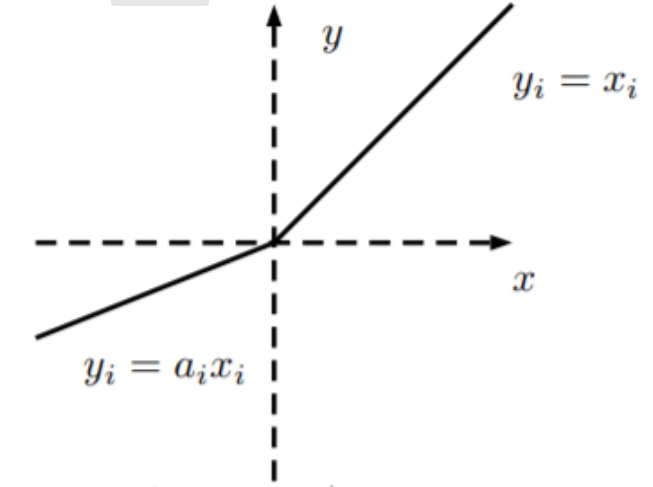
\includegraphics[width=0.9\columnwidth]{photo/leakyrelu}
\caption{A visual representation of the leaky Linear rectified unit (Leaky-ReLU) $\cite{xu2015empirical}$}
\label{fig:leakyRelu}
\end{figure}

A leaky ReLU layer operates based on a threshold operation, any input value less than zero is multiplied by a fixed scalar a. This operation is equivalent to:
\begin{align}
   & \large \large \ y_{i} = \begin{cases} x_{i}, & x_{i}\geq 0 \\ \frac{x_{i}}{a_{i}}, & x_{i}< 0. \end{cases}
\end{align}
Where $a_{i}$ is a fixed parameter in range (1, +\infty).\hfill

\textbf{Dropout}\\

Dropout is a stochastic regularization technique introduced by \cite{srivastava2014dropout}, it works by adding noise to its hidden units to regularize the neural network. Some neurons are neglected throughout training. This indicates that any weight updates are not applied to the neuron on the backward pass and their contribution to the activation of downstream neurons is removed temporally on the forward pass \cite{brownlee_2017}. Resulting in a less sensitive network to the specific weights of neurons. This, in turn, makes the network less likely to overfit the training data and results in a system that is proficient of better generalization.
In our model, we applied dropout in the training phase to prevent over-fitting. Although dropout prevents any type of over-fitting and delivers far more robust models, the system’s learning will eventually slow down in case of the high amount is being added to the network during training, in our experience, we dropped 20\% of the hidden layers to activate other neurons and making them handle the required representation to make predictions for the dropped neurons. Setting the dropout to this value prevents the distribution from getting a high variance, otherwise, the model will over-fit during training. As a result, the network will learn multiple independent internal representations after every iteration. A representation of the dropout model is shown in Figure \ref{fig:dropout}.



\begin{figure}[]
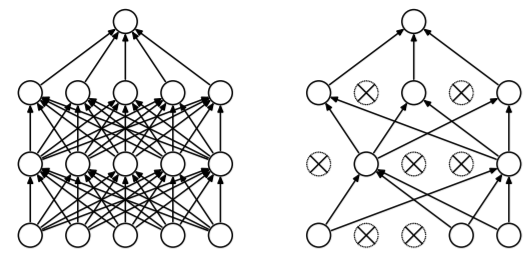
\includegraphics[width=0.98\columnwidth]{photo/do}
\caption{Left: A standard multi-layer perceptron with 2 hidden layers. Right: An example of the same network produced by applying dropout, in this case their crossed units have been dropped from the hidden layer $\cite{srivastava2014dropout}$}
\label{fig:dropout}
\end{figure}\hfill

\textbf{Model Parameters}\\

In our CNN model, each layer has two types of parameters: weights and biases. The total number of parameters is the sum of all weights and biases. These parameters are essential because they are directly correlated with the model performance and accuracy, and having many parameters will make the network flexible enough to represent the desired mapping and allow us to employ stronger regularization to prevent over-fitting. We calculated these two parameters according to the following formulas in \cite{mallik_2018}. \\

\textbf{For a convolutional layers:}\\
\begin{align}
   & Conv 3D=\begin{cases}
\large W_{c} = O^{2} \ast N \ast F, \\
\large B_{c} = F\,\\
\large P_{c} = W_{c} + B_{c}\
\end{cases}
\end{align}


\textbf{For fully connected layers:}\\
\begin{align}
   & FC Layer=\begin{cases}
\large W_{cf} = O^{2} \ast N \ast F, \\
\large B_{cf} = F\,\\
\large P_{cf} = W_{cf} + B_{cf}\
\end{cases}
\end{align}


where \textbf{W} represent number of weights, \textbf{O} is the size of the output image, \textbf{N} is the number of kernels, \textbf{F} is the number of filter, \textbf{B} is the number of biases, and \textbf{P} is the number of parameters.
There are no parameters associated with the max pooling layer and dropout. The calculated values of these numbers are listed in Table \ref{tab:CNN}, and Figure \ref{fig:modelarchitecturecnn} visualize the full architecture of the proposed CNN model.

\begin{table}[]
\caption{Total number of parameters in our proposed neural network architecture.}
\centering
\begin{tabular}{|c|c|c|c|c|}
\hline
\textbf{Layer  name} & \textbf{Image} & \textbf{Weight} & \textbf{Biases} & \textbf{Params} \\ \hline
Input image & 128x128x1 & 0 & 0 & 0 \\ \hline
Conv3D & 126x126x64 & 576 & 64 & 1792 \\ \hline
MaxPool3D & 63x63x64 & 0 & 0 & 0 \\ \hline
Conv3D & 61x61x128 & 1152 & 128 & 221312 \\ \hline
MaxPool3D & 31x31x128 & 0 & 0 & 0 \\ \hline
Conv3D & 29x29x256 & 2304 & 256 & 884,992 \\ \hline
Conv3D & 27x27x256 & 2304 & 256 & 1,769,728 \\ \hline
MaxPool3D & 14x14x256 & 0 & 0 & 0 \\ \hline
Conv3D & 12x12x512 & 0 & 0 & 0 \\ \hline
MaxPooling3D & 6x6x512 & 0 & 0 & 0 \\ \hline
GAP & 512x1 & 0 & 512 & 0 \\ \hline
Dense & 4,096x1 & 4,096,000 & 4,096 & 2,101,248 \\ \hline
Dropout & 4,096x1 & 0 & 4,096 & 0 \\ \hline
Output & 6 & 0 & 0 & 24582 \\ \hline
Total Params & \multicolumn{4}{c|}{8,543,110} \\ \hline
\end{tabular}
\label{tab:CNN}
\end{table}\hfill

\textbf{Global Average Pooling (GAP)}\\

From the total number of parameters table \ref{tab:CNN}, we can perceive that the number of parameters is progressively increasing after each layer and architecture like this has the uncertainty of overfitting to the training dataset. As mentioned in \cite{lin2013network} and \cite{zhou2016learning}, GAP layer works remarkably well in diminishing the spatial dimension of the output representation of the data. For this reason, we chose to use a GAP layer that comes before the fully connected layer to minimize over-fitting. As an example, the number of parameters in our model is reduced from 3,539,456 to 2,101,248 after applying GAP layer, which also indicates that the dimensions hxwxd of our input image are reduced in size to have dimensions 1x1xd. GAP layers reduce each h×w feature map to a unique number by solely taking the average of all hxw values.\\


\textbf{Model architecture}\\

The CNN network structure consists of 5 convolutional layers each with a 3x3 filter with a stride of 1, and 4 max-pooling layers each with 2x2 filter and stride of 1, after the max pooling layer, we applied a GAP layer to reduce the parameters and prevent over-fitting. Then we applied 1 dense layer with 4096 neurons was added with Leaky-RelU that has an alpha angle of 0.2. During training, in each iteration, the network randomly drops out 20\% of the neurons prior to the fully connected layer. Lastly, a softmax layer was added to map the compressed motion information to 6 action classes. Number of filters started with 64 for the first
3D convolutional layer and gradually increases to 512 before the fully connected layers. Table illustrates the layers name and spatial dimensions.  
\begin{figure*}[ht]
\centering
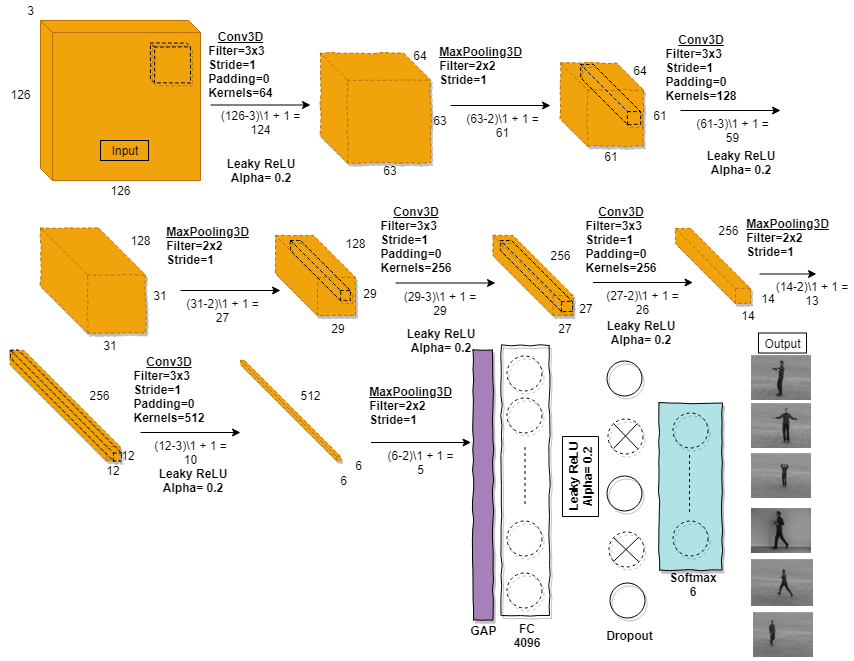
\includegraphics[width=1.5\columnwidth]{photo/nn2}
\caption{3D CNN contains: 5 3D convolution, 4 MaxPooling, 2 fully connected layer, and 1 softmax output layer. All convolution kernels are of size 3x3x3 with stride of 1. Number of filters start with 64 for the first 3D convolutional layer and gradually increase to 512 before the fully connected layers. All pooling kernels are 2x2x2. Each fully connected layer has 4096.}
\label{fig:modelarchitecturecnn}
\end{figure*}

\subsubsection{Recurrent Convolutional Neural Network} \label{ewlu}
A recurrent neural network can handle a sequence of information with a varied length of time steps. \textbf{$h_{t}$} is the internal hidden state, generated as a result of transformation on the input \textbf{X} at every iteration. The network transfers the state \textbf{$h_{t}$} along with the input \textbf{$X_{t+1}$} to the neuron after every time step. The network then learns to remember and forget information with a non-linear activation function. The whole process happens once we apply Equation \ref{eq:equ1} and Equation \ref{eq:equ2} to the system.
\begin{align}
\label{eq:equ1}
   &\large h_{t}=\sigma (W\binom{x_{t}}{h_{t-1}})
\end{align}

\begin{align}
\label{eq:equ2}
   &\large y_{t}=\sigma (V*h_{t})
\end{align}

Where $\textit{t}$ represents time steps, and \textbf{W} and \textbf{V} are respectively the weights and biases for the layer, and $\sigma$ represents the non linear activation function which in our case, is a rectified linear unit introduced by Geoffrey \textit{et al.} in 2010 \cite{nair2010rectified} with R(\textit{z})=max(0,\textit{z}) same as ReLU in Activation function.\\

\textbf{Long Short Term Memory (LSTM)}\\

Mathematically, the network complexity increases when multiple layers of RNNs are stacked, which create the problem of vanishing gradient as the RNN doesn't memorise information over a longer time. This problem is solved by adding a long short term memory layer (LSTM) \cite{hochreiter1997long} which store information in gated cells at the neurons. This allows errors to be back-propagated through many time steps.
\begin{align}
   & \left ( i \right ) = \left ( sigm \right ) W\binom{x_{t}}{h_{t-1}}
\end{align}

\begin{align}
   & \left ( f \right ) = \left ( sigm \right ) W\binom{x_{t}}{h_{t-1}}
\end{align}

\begin{align}
   & \left ( o \right ) = \left ( sigm \right ) W\binom{x_{t}}{h_{t-1}}
\end{align}

\begin{align}
   & \left ( \hat{c_{t}} \right ) = \left ( tanh \right ) W\binom{x_{t}}{h_{t-1}}
\end{align}

\begin{align}
   & c_{t}=f\odot c_{t-1}+i\odot \hat{c_{t}}
\end{align}

\begin{align}
   & h_{t}=o\odot tanh \left (c_{t}\right )
\end{align}

where \textbf{i}, \textbf{f} and \textbf{o} are the input gate, forget gate and output gate, $\hat{c_{t}}$ represents new state value, which can be added to the cell state $c_{t}$. We used $\odot$ for elemen-twise multiplication.\\

\textbf{Activation Function - ReLU}\\

The Linear rectified unit (ReLU) function is introduced by Geoffrey \textit{et al.} in 2010 \cite{nair2010rectified}. It gives a 0 as an output
when x $\geq$ 0, and then produces a linear with slope of 1 when x $\leq$ 0 (refer to Figure \ref{fig:relufunction} for visualization).
Mathematically, it's defined as R(\textit{z})=max(0,\textit{z})\label{eq:111}. It was demonstrated to further improve the training of any types of neural networks. Visually, it looks like the following:\\


\begin{figure}[ht]
\centering
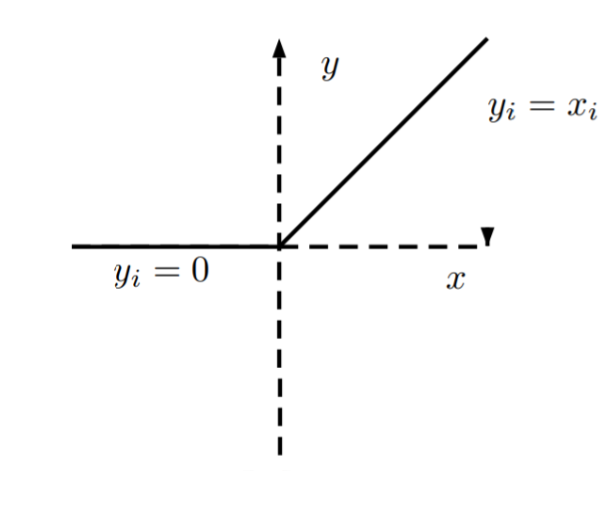
\includegraphics[width=0.7\columnwidth]{photo/relufunction.PNG}
\caption{A visual representation of the Linear rectified unit (ReLU) \cite{nair2010rectified}.}
\label{fig:relufunction}
\end{figure}

\begin{align}
   & \large \large \ y_{i} = \begin{cases} x_{i}, & x_{i}\geq 0 \\ 0, & x_{i}< 0. \end{cases}
\end{align}

This function changes all negative activations to 0 as a threshold and all other values are unchanged. ReLU introduces non-linearity properties of the model without affecting the receptive field of the convolutional layer. It also speeds up the neural networks training and avoiding vanishing gradient problem. Refer to Figure \ref{fig:relufunction} for visual representation.\\ 

\textbf{Batch Normalization}\\

During training, it has been reported by  \cite{ioffe2015batch} that the internal covariate shift makes the training process of the network extremely slow and infficient. The covariate shift is the distribution of the variations in the input layer during training due to the parameters grow in the previous layer. We could avoid the internal covariate shift by whitening the activations layer, but this process is computationally expensive. Batch normalization, a part of our neural network composition, approximates this process by regulating the activations using a statistical measure of the mean $\widehat{E}(x)$, and standard deviation $\widehat{Var}(x)$  for each mini batch training. Formula \ref{eq:batch} which was introduced by \cite{ioffe2015batch} describes the batch normalization process.

\begin{align} \label{eq:batch}
   & \large BN\left ( x;\gamma ,\beta \right )=\gamma \frac{x-\widehat{E}(x)}{\sqrt{\widehat{Var}(x)+\epsilon }} +\beta
\end{align}

Where $\gamma$ and $\beta \in \mathbb{R}^{d}$ are scale and shift parameters for the activation $x \in \mathbb{R}^{n*d}$, $d$ is \in (1,+$\infty$). An identity transformation is then presented for each activation. $\epsilon \in \mathbb{R}$ is a constant added as a regularization parameter for numerical stability. In the BN equation above, the division is performed element-wise. $\gamma$ and $\beta$ are learned during training and fixed during inference.\\

\textbf{Model Architecture}\\

We implemented a CNN network fused with 2 main RNN layers, to improve the model performance. The additional RNN network is acting as a memory layer to the network. Since the data consists of a sequence of videos, a convolutional model with memory layers is used to learn spatiotemporal features from the videos.

In this case, we only took 40 frames from the middle of each video. These frame sequences are the input of the convolutional network that consists of 1 convolutional layer with 3x3 filters and a stride of 1,  a batch normalization layer is applied to standardizes the recurrent network from its activations function, we then apply the activation function ReLU, then we add a max pooling layer with filter of 2x2 and stride of 1 and finally a dropout layer that drops 25\% of the hidden layer during training. This architecture is repeated three times as shown in figure \ref{fig:cnnlstm}. We then add 2 fully connected layer with 256 and 128 neurons respectively. Before applying any RNN layer, we wrapped the whole network with "Time distributed" layer that acts the same as a fully connected layer to every time step of a 3D tensor. The second part of the network is a many to one RNN network because the model is converting a sequence of video to one single prediction. For that reason, we applied 2 LSTM layer, each has an input dimension of 128 with Tanh activation function and 256 output dimension. After this operation, we have concatenated these layers into one and we apply the softmax operation that holds all the human action labels.

\begin{figure*}[h]
\centering
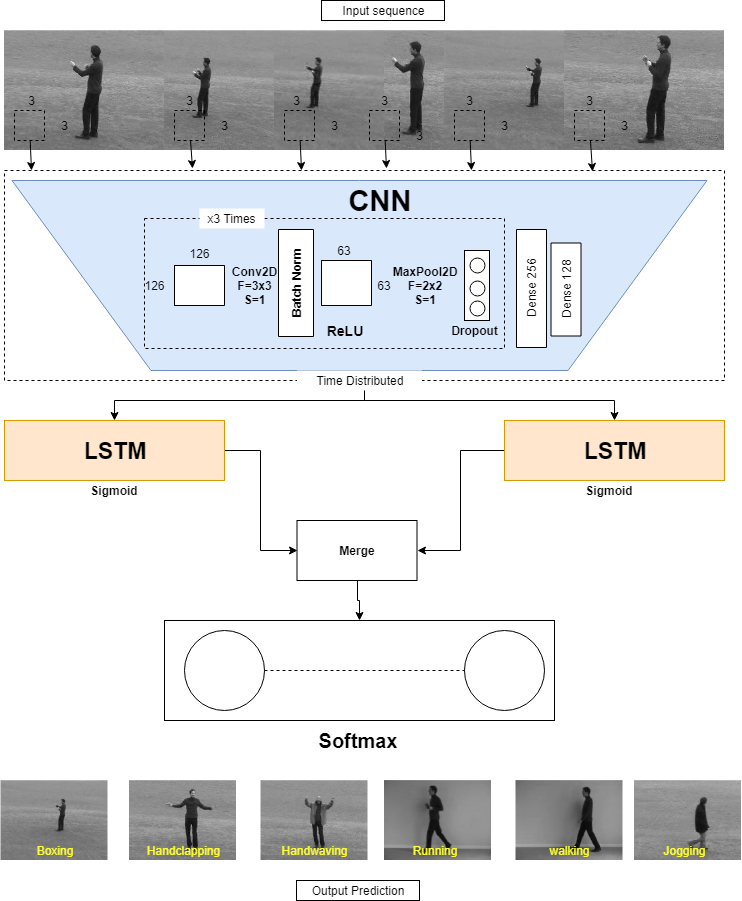
\includegraphics[width=1.3\columnwidth]{photo/cnnlstm.png}
\caption{CNN-LSTM contains: 1 2D convolution,1 Batch Norm, 1 MaxPooling, a Relu function, and 1 Dropout layer, all of them are repeated 3 times, then 2 dense layers with 256 and 128 neurons. There 2 long  short term memory channels, both with inner Tanh function, and 256 output dimension.}
\label{fig:cnnlstm}
\end{figure*}

\subsection{Training and Testing}
We first introduced the dataset, then we described the setup and parameter settings for the experiments. We use the same training for both of these models. The validation set is divided for 16\% and 50\% for the training set and the rest is left for testing.
For optimization, we applied the Stochastic gradient descent (SGD) process with momentum to update model parameters $theta$ in the negative direction of the gradient $g$ by taking a mini-batch of data of size $m$. SGD is applied by using Equation \ref{eq:equ3} below.

\begin{equation}
\label{eq:equ3}
    \arge g=\frac{1}{m}\Delta _{\Theta }\sum _{i}L(f(x^{(i);\Theta }), y^{(i)})
\end{equation}

On large dataset, SGD performs updates more frequently because it has the ability to converge faster than the batch training. , another reason for this selection is our videos contain lots of redundant frames, the gradient can reasonably approximate these redundancies without using the full dataset. For our model, we manipulated the moving average of our gradient descent by defining a specific momentum. We used this momentum to update the weight and the bias of the model, and we used to the formula below: 
\begin{align}
   & \large V_{t}=\beta V_{t-1}+(1-\beta )\Delta wL(W,X,y)
\end{align}
\begin{align}
   & \large W=W-\alpha V_{t}
\end{align}

Where \textbf{L} is the loss function,  \textbf{$\delta$} is the gradient, \textbf{$\alpha$} is the learning rate and \textbf{W} is the model weight.
For both models, we used Keras and Scikit-learn to build the network and we run the experiments on NVIDIA Geforce 1050i Titan GPU.
For the first proposed CNN model, we set the learning rate to 0.0001 with 0.9 momentum and 0 decay. We trained to network from scratch using mini batches of 128 over 100 epochs.
For the second proposed CNN-RNN model, we set the learning rate to 0.01 with 0.9 momentum and $10^{-5}$ decay. We also use 32 mini batches and trained to network from scratch over 100 epochs.

\section{Results and discussions}
After training both of the models on the given dataset, we have decided to use three of the evaluation matrices, such Confusion matrix, Accuracy and Cross entropy loss function. Below we presented each of these evaluation metrics with their associated results.\\


\begin{center}
    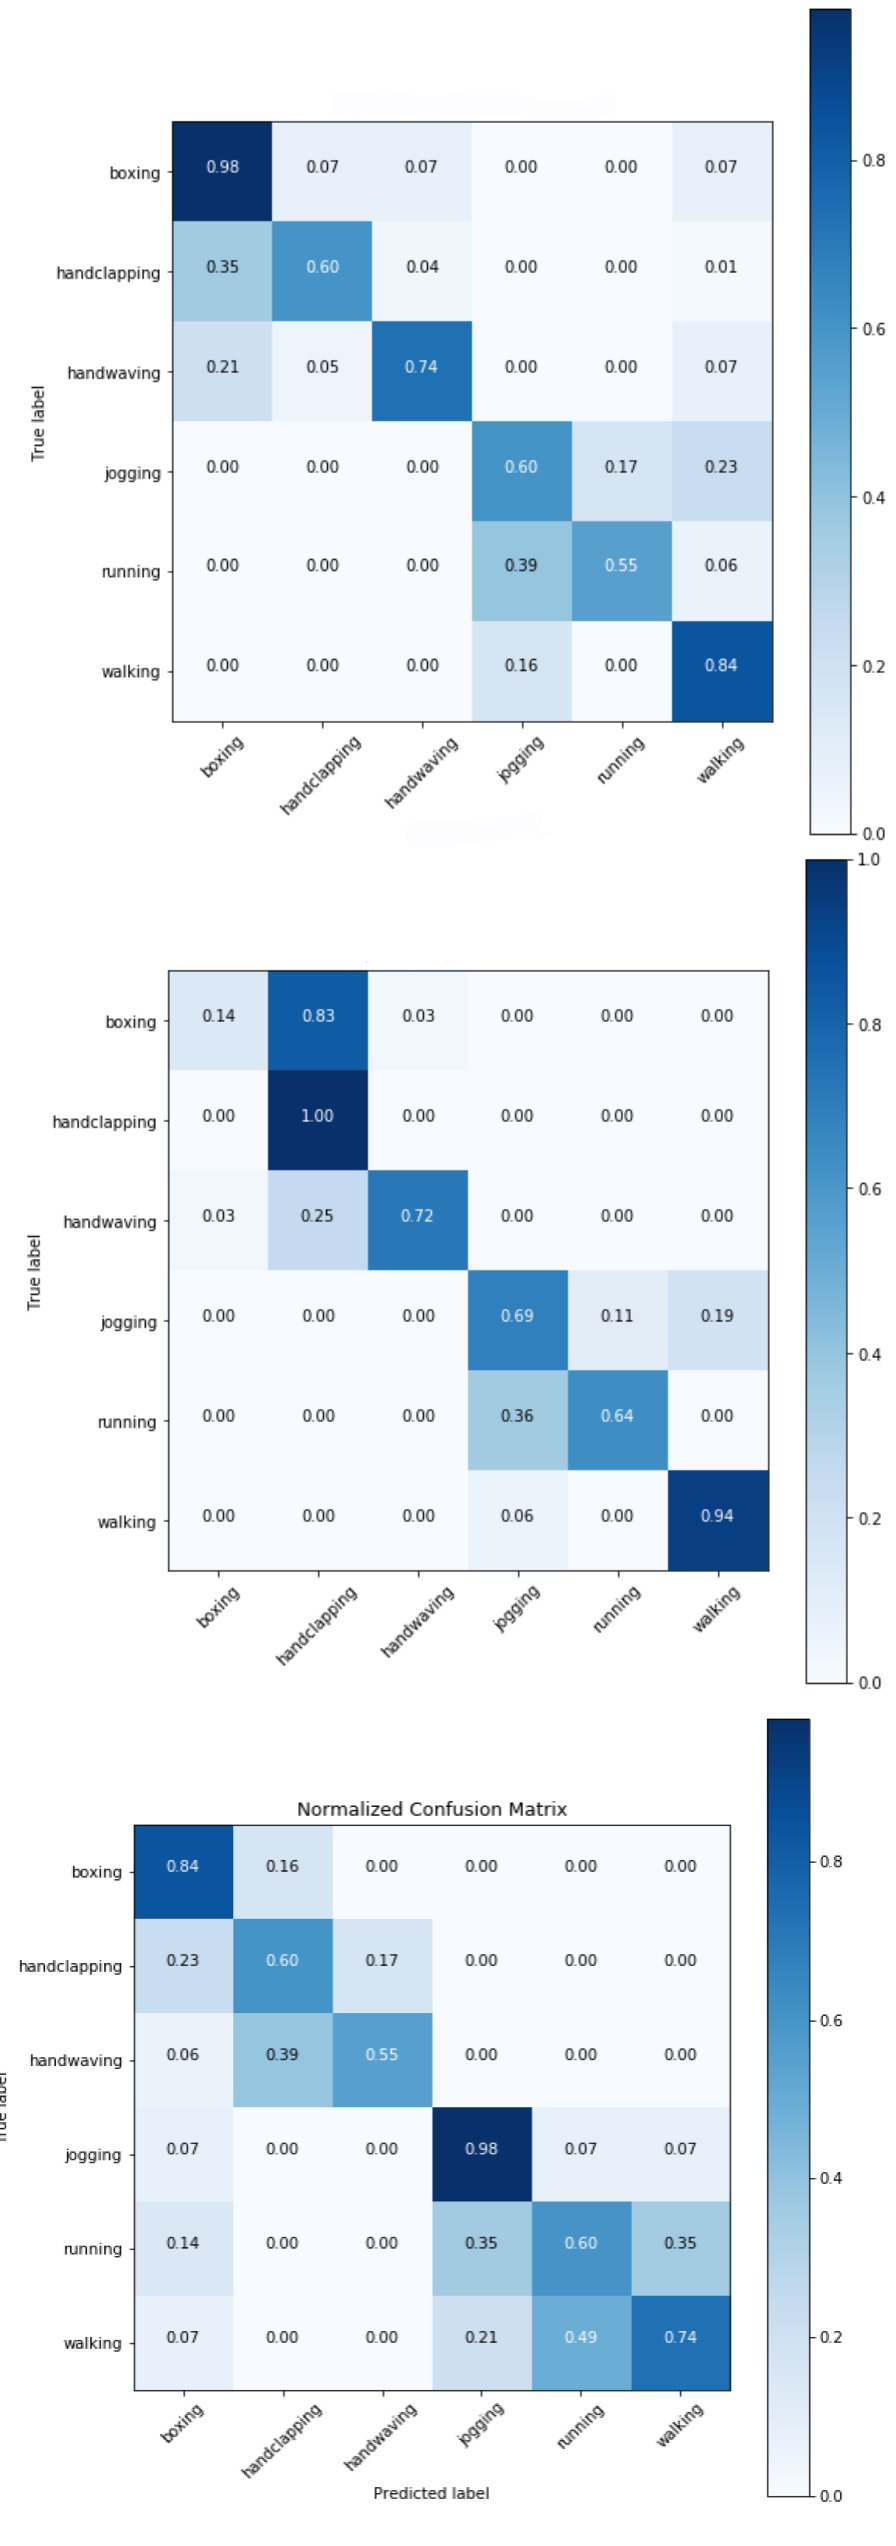
\includegraphics[width=0.4\textwidth]{photo/m.jpg}
\captionof{}{\textbf{Figure 7: Top: Confusion matrix for the CNN-LSTM model. Middle: Confusion matrix for the CNN model. Bottom: Confusion matrix for benchmark results.}}
    \label{fig:mc-1}
\end{center}

The confusion matrix visualized in Figure 7 was implemented by randomly selecting 9 different persons, processed all the videos of these 9 persons where 9x4=216 videos and constructed the confusion matrix using the proposed models. We provided a summary of the confusion matrix results in Table \ref{confusionmatrixtable}. In case of Boxing, when the actual label was "Boxing" our CNN-LSTM model predicted 98\% of the time, whereas the benchmark model predicted it 84\% of the time, that's an improvement of 14\% over the benchmark resutls. However, the benchmark results showed a confidence of 98\% for action like jogging, whereas our model achieved only 69\% and 60\%. Overall, our proposed CNN model achieved higher predictions on action like Walking (94\%), Handclapping (100\%) and Running (64\%), and the proposed CNN-LSTM achieved higher prediction on Handwaving (74\%) and Boxing (98\%).\\

Accuracy was achieved by adding the total number of true positives with the total number of true negative and dividing them over the total number of data.
\begin{align}
   & \large Acc=\frac{TP + TN}{TD}
\end{align}
where \textbf{TP} are the True positive, \textbf{TN} are the true negative and the \textbf{TD} are total number of data.

We have used the cross entropy loss function \cite{zhang2018generalized} to measure the performance of the neural network. Cross-entropy increases as the predicted probability diverge from the actual label. For instance, a perfect model will have a 0 loss. It was achieved and calculated from Equation \ref{cross}.
\begin{align} \label{cross}
    & H(y,\widehat{y}) = \sum_{i}y_{i}log\frac{1}{\widehat{y_{i}}}
\end{align}


\begin{table}[h]
\centering
\caption{Comparison between both of our proposed
model.}
\begin{tabular}{|c|c|c|c|c|}
\hline
\textbf{Model name} & \textbf{Accuracy} & \textbf{Loss} & \textbf{Layers} & \textbf{Parameters} \\ \hline
\textbf{CNN}        & 64.76\%            & 0.823         & 13              & 8,543,110           \\ \hline
\textbf{CNN-LSTM}   & 92.23\%            & 0.087         & 18              & 1,657,792           \\ \hline
\end{tabular}
\label{accuracyloss}
\end{table}\\



\begin{table}[ht]
\centering
\begin{tabular}{|c|c|c|c|}
\hline
\textbf{Action} & \textbf{CNN model} & \textbf{CNN-LSTM} & \textbf{Benchmark} \\ \hline
\textbf{Walking} & \textbf{94\%} & 84\% & 74\% \\ \hline
\textbf{Jogging} & 69\% & 60\% & \textbf{98\%} \\ \hline
\textbf{Handclapping} & \textbf{100\% }& 60\% & 60\% \\ \hline
\textbf{Handwaving} & 72\% & \textbf{74\%} & 55\% \\ \hline
\textbf{Running} & \textbf{64\%} & 55\% & 60\% \\ \hline
\textbf{Boxing} & 14\% & \textbf{98\%} & 84\% \\ \hline
\end{tabular}
\caption{Represents a summary of the results taken from the confution matrix.}
\label{confusionmatrixtable}
\end{table}\\



In Figure 7, 8, 9 and 10, we visualized both of the CNN and CNN-LSTM accuracy and loss for training and test set. Results and visualizations show that the accuracy for the CNN-LSTM appeared to be more consistent with a maximum accuracy of 92.23\% for the training set and 61.2\% for the test set over 100 epochs. Whereas, the accuracy of the CNN model appeared to be inconsistent, where spikes appeared after each iteration which clearly indicates an over-fitting pattern and high variance for the test set, at the $90^{th}$ epoch the accuracy for the training set is 64.76\% and 59\% for the test set. On the other hand, the loss results for CNN-LSTM appeared to have low bias and high variance, due to the difference between the train and test set. The model has 0.087 loss for a train set and 2.04 loss for the test set. However, the loss for the CNN model shows a consistent pattern for the train set and a large spike for the test set at the $78^{th}$ epochs. This model has 0.823 loss for training and 1.3 loss for the test set. This implementation proves that adding LSTM layers works well with sequential video data and help in improving the model performance. We also notice that the number of layers and the number of parameters are correlated with the accuracy of the model. We had more accuracy with fewer parameters and more layers.
\begin{figure*}[ht] 
  
  \begin{minipage}[b]{0.5\linewidth}
    \centering
    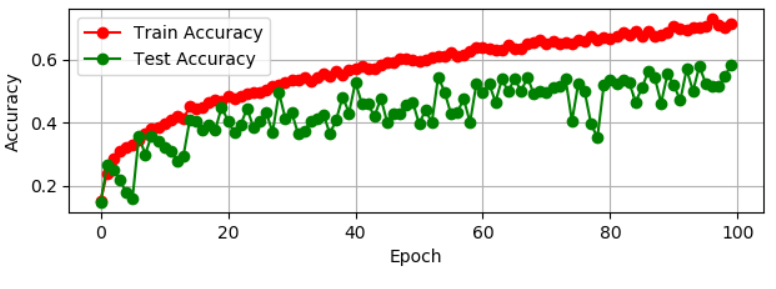
\includegraphics[width=1\linewidth]{photo/cnnaccuracy.PNG} 
    \caption{Accuracy plot for the CNN model.}
    \label{fig:b}
    \vspace{4ex}
  \end{minipage}%%
  \label{fig:7869}
  \begin{minipage}[b]{0.5\linewidth}
    \centering
    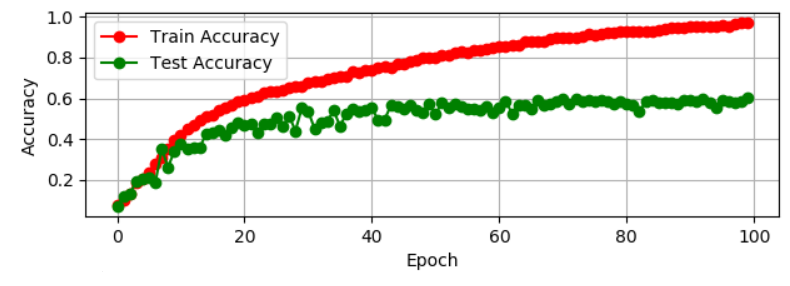
\includegraphics[width=1\linewidth]{photo/cnnlstmaccuracy.PNG} 
    \caption{Accuracy plot for the CNN-LSTM model.} 
    \vspace{4ex}
  \end{minipage} 
  \begin{minipage}[b]{0.5\linewidth}
    \centering
    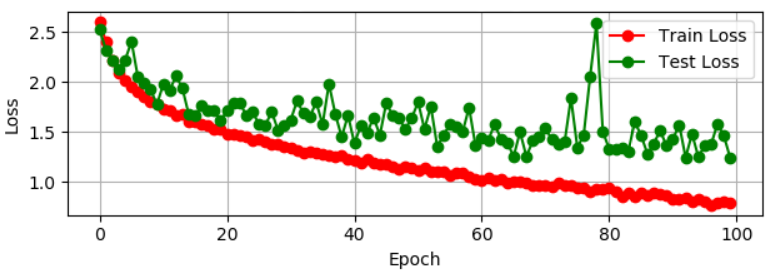
\includegraphics[width=1\linewidth]{photo/cnnloss.PNG} 
    \caption{Loss plot for the CNN model.} 
    \vspace{4ex}
  \end{minipage}%% 
  \begin{minipage}[b]{0.5\linewidth}
    \centering
    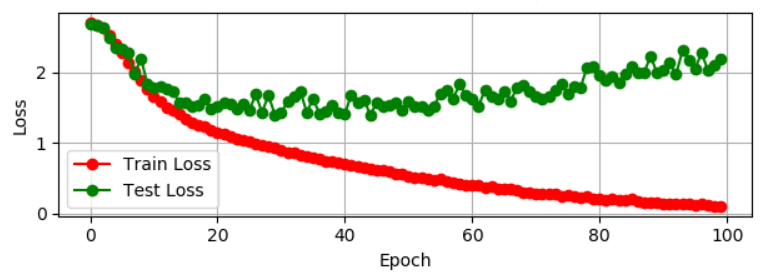
\includegraphics[width=1\linewidth]{photo/cnnlstmloss.PNG}
    \caption{Accuracy plot for the CNN-LSTM model.} 
    \vspace{4ex}
  \end{minipage} 
\end{figure*}\label{fig:fig7868} 



\begin{figure}[ht]
\centering
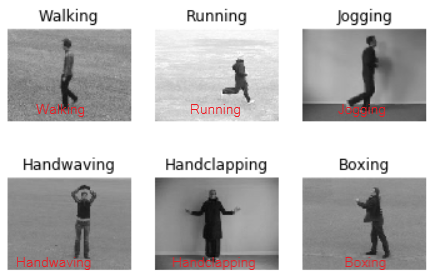
\includegraphics[width=0.8\columnwidth]{photo/classified.png}
\caption{Visualization of the correctly classified action samples. We used to model weight after training to predict action labels from random videos. These predictions were random picked from CNN and CNN-LSTM models.}
\label{fig:classified}
\end{figure}\\

\begin{figure}[h]
\centering
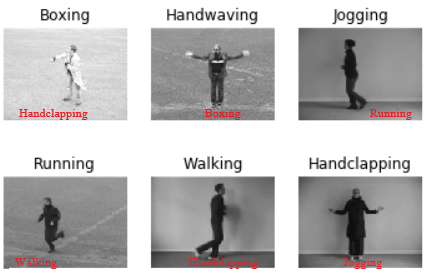
\includegraphics[width=0.8\columnwidth]{photo/missclassified.png}
\caption{Visualization of the miss classified action samples. We used the model weight after training to predict action labels from random videos. These predictions were randomly  picked from CNN and CNN-LSTM models.}
\label{fig:missclassified}
\end{figure}

In Figure \ref{fig:classified} and Figure \ref{fig:missclassified}, we presented some of the correctly classified and miss-classified action samples. These samples are randomly picked from the featured CNN and CNN-LSTM model prediction results. Both of the networks was able to correctly predict the action, however, it sometimes failed to predict the correct action.
There could be various reasons for this observation. Based on these observations and results, there are several reasons. First, human actions are naturally confusing. Secondly, there are imperfections in the data due to variation in light and scale. Thirdly, our CNN models are trained on a dataset that is considered small to other big datasets such as Youtube or HMBD etc. One way to solve this issue is by using more GPU memory and computing power and using more video data.
%\end{document}  % This is where a 'short' article might terminate

% ensure same length columns on last page (might need two sub-sequent latex runs)
\balance

%ACKNOWLEDGMENTS are optional
\section{Conclusion}
Human action recognition is still considered a hard task, despite the notable discoveries over the past three decades. This is expected because actions are not well defined enough like object in a dynamic scene such as videos. An action recognition system needs more context about the image, and they are affected by the low-quality data, background noise, intra-class variability and action complexity.

In this paper, we proposed two neural network structures that help in recognizing the most common human actions from a sequence of videos. The convolutional neural network model learned from the visual appearance of each action and classified these appearances to 6 actions label with an accuracy of 64.76\% with 13 network layers and 8.54 million parameters. While the second model has an additional LSTM layer that remember and forgets recurrent gates for every frame in the video. This model achieved an accuracy of 92.23\% with 18 layers and approximately 1.65 million parameters. Results of CNN-LSTM method are 27.47\% higher than using the proposed CNN layers alone. In the end, we conclude that a high accuracy model can be achieved by using a deeper neural network with more layers using less complex structures.



% The following two commands are all you need in the
% initial runs of your .tex file to
% produce the bibliography for the citations in your paper.
\bibliographystyle{abbrv}
\bibliography{vldb_sample}  % vldb_sample.bib is the name of the Bibliography in this case
% You must have a proper ".bib" file
%  and remember to run:
% latex bibtex latex latex
% to resolve all references


%APPENDIX is optional.
% ****************** APPENDIX **************************************
% Example of an appendix; typically would start on a new page
%pagebreak
\end{document}
